\documentclass[a4paper,12pt,ruledheader,onecolumn,ceqn]{article}
%a4paper -> página no formato A4
%12pt -> letra padrão tamanho 12
%ruleheader -> coloca uma linha sublinhando o cabeçalho
\usepackage{abntcite}
\usepackage{amsmath,amsfonts,amsthm}  %pacote para equações
\usepackage[utf8]{inputenc}			  %encoding utf8
\usepackage[brazil]{babel}            %pacote de idioma
\usepackage{here}                     %exige que a figura fique no local especificado (utilizar [H])
\usepackage{url}                      %para trabalhar com URL's no texto
\usepackage{makeidx}                  %para fazer índice remissivo
\usepackage{multirow}                 %para fazer alterações nas tabelas
\usepackage{caption}                  %para fazer alterações nas legendas
\usepackage{array}
\usepackage{indentfirst}			  %inserir parágrafo
\usepackage[titles]{tocloft}          %para alinhar o Sumário (Alinhamento à Esquerda) 
\usepackage{tocloft, blindtext}       %para permitir alterações nas figuras e tabelas
\usepackage{graphicx}                 %permite colocar figuras
\usepackage{epstopdf}				  %converte eps em pdf	
\usepackage{wrapfig}                  %permite posicionar figuras
\renewcommand{\cftfigpresnum}{Figura }      %para colocar a palavra "Figura" na lista de figuras,
%antes do número e identar corretamente
\renewcommand{\cfttabpresnum}{Tabela }      %para colocar a palavra "Tabela" na lista de tabelas,
%antes do número e identar corretamente

\let\oldthebibliography=\thebibliography    % Para controlar os espaços entre os itens da referência  
\let\endoldthebibliography=\endthebibliography
\renewenvironment{thebibliography}[1]{%
	\begin{oldthebibliography}{#1}%
		\setlength{\parskip}{0ex}%
		\setlength{\itemsep}{2ex}%
		\setlength{\topskip}{-20ex}%
	}%
	{%
	\end{oldthebibliography}%
}

%definindo as marges 
\usepackage{geometry}
\geometry{top=20mm,bottom=20mm,left=20mm,right=20mm}

%\counterwithout{equation}{chapter}          %serve para enumerar as equações sequencialmente 
%(usa o pacote chngcntr)
\DeclareCaptionLabelSeparator{colon}{ - }   %serve para colocar o hifen na legenda da figura 
%(exemplo: Figura 1 - Visão geral...) (usa o pacote caption)
\captionsetup{textfont=small}               %padroniza o tamanho da legenda da figura para "small"
\captionsetup{labelfont=small}              %padroniza o tamanho do título da figura para "small"

\DeclareCaptionLabelSeparator{fill-newline}{\hfill\null\par}

\captionsetup{%
	format=hang,
	labelformat=simple,
	%labelsep=fill-newline,
	singlelinecheck=false,
	justification=centering,
	position=top,
}

%------colocando niveis de subsecoes------------------------------------------
\setcounter{secnumdepth}{4}                   %numero de subsecoes
\setcounter{tocdepth}{4}                      %numero de subsecoes no sumario

%------se tiver problema com a hifenização de alguma palavra)
%\hyphenation{ En-gen-nha-ri-a com-pu-ta-ção } 
%---sem hifenização
\usepackage[none]{hyphenat}
\sloppy

%%%%%%%%%%%%%%%%% Para alterar o tipo de letra da seção, subseção e subseção %%%%%%%%%%%%%%%%%
\makeatletter
%\def\l@section#1#2{\pagebreak[3]
%\vskip 0.0em plus 0pt  % space above chapter line
%\@tempdima 1.3cm       % width of box holding chapter number
%\begingroup
%\parindent \z@ \rightskip \@pnumwidth
%\parfillskip -\@pnumwidth
%%\bfseries\textsc     
%\fontfamily{cmss}\fontseries{sbc}\selectfont % Boldface removed. 2006nm %% <= \bfseries uncommented again
%\leavevmode          % TeX command to enter horizontal mode.
%#1\hfil \hbox to\@pnumwidth{\hss #2}\medskip\par%% <= \medskip inserted
%\endgroup}

\def\l@subsection#1#2{\pagebreak[3]
	\vskip -0.2em plus -1pt  % space above chapter line
	\@tempdima 1.3cm       % width of box holding chapter number
	\begingroup
	\parindent \z@ \rightskip \@pnumwidth
	\parfillskip -\@pnumwidth
	%\bfseries\itshape    
	\fontfamily{ptm}\bfseries\selectfont % Boldface removed. 2006nm %% <= \bfseries uncommented again
	\leavevmode          % TeX command to enter horizontal mode.
	#1\hfil \hbox to\@pnumwidth{\hss #2}\medskip\par%% <= \medskip inserted
	\endgroup}

\def\l@subsubsection#1#2{\pagebreak[3]
	\vskip -0.2em plus -1pt  % space above chapter line
	\@tempdima 1.3cm       % width of box holding chapter number
	\begingroup
	\parindent \z@ \rightskip \@pnumwidth
	\parfillskip -\@pnumwidth
	%\fontseries{b}                
	\fontfamily{ptm}\bfseries\itshape\selectfont % Boldface removed. 2006nm %% <= \bfseries uncommented again
	\leavevmode                 % TeX command to enter horizontal mode.
	#1\hfil \hbox to\@pnumwidth{\hss #2}\medskip\par%% <= \medskip inserted
	\endgroup}
\makeatother
%%------------------------------------------------------------------------------------------
\usepackage{rotating,booktabs}
\def\MC#1{\multicolumn{1}{c}{#1}}
%%------------------------------------------------------------------------------------------
\newcommand{\HorRule}[1]{\noindent\rule{\linewidth}{#1}} 

\title{	
	\normalfont \normalsize 
	\Large \textbf{Universidade do Oeste de Santa Catarina} \\ %Universidade e departamento
	\large Engenharia Elétrica \\ [0.1cm] %Universidade e departamento
	\HorRule{1.5pt} \\ 			%linha fina horizontal
	\textbf{Título} \\ 			%título da atribuição
}
\author{Autor 1 \\
	Autor 2}                    %nome de um ou mais autores

\date{\normalfont\today}    %O dia ou customizar a data



\begin{document}
%%%%%%%%%%%%%%INÍCIO DO CABEÇALHO%%%%%%%%%%%%%%
\begin{wrapfigure}[2]{l}{3cm}
\vspace{-0.4cm}

\includegraphics[scale=0.4]{figuras/eletrica.jpg}
\end{wrapfigure} 

\hspace*{1.2cm} \textbf{UNIVERSIDADE DO OESTE DE SANTA CATARINA} \\
\hspace*{2.1cm} \textbf{ÁREA DE CIÊNCIAS EXATAS E TECNOLÓGICAS} \\
\hspace*{8.0cm} Curso de Engenharia Elétrica 

\HorRule{1.0pt}  			%linha fina horizontal
\begin{center}
\large\textrm{\textbf{MODELO DE RELATÓRIO - ACET UNOESC \\ ENGENHARIA ELÉTRICA}} 
\end{center}

\vspace{0.5cm}
\hspace{-1.05cm}
$\left. \begin{array}{ll} 
\mbox{24384} & \mbox{Kleyton Hoffmann} \\
\mbox{código} & \mbox{Nome} \\
\end{array} \right.$

\HorRule{1.0pt}  			%linha fina horizontal
%%%%%%%%%%%%%%FIM DO CABEÇALHO%%%%%%%%%%%%%%


\section{Introdução}

Com a necessidade contínua de promover aperfeiçoamento nos trabalhos acadêmicos do curso de Engenharia Elétrica, buscou-se a ferramenta \LaTeX \cite{abntex2modelo} para criar um ambiente favorável de padronização. Está padronização pode-se propagar em outros cursos da UNOESC, bem como profissionais de áreas diversas que possuem problemas de padronização de documentos. Essa padronização está de acordo com \citeonline{livro-unoesc}. 

\subsection{Objetivos}

\subsubsection{Objetivo Geral}

Ao final do curso o acadêmico irá ter a possibilidade de padronizar seus documentos, evitando publicações desconfiguradas e sem padrões.

\begin{figure}[ht!]
	\centering
	\caption{Modelo de um circuito trifásico \label{Fig:circuito1}}
	\vspace{-0.5cm}
	%fasdfasdf
	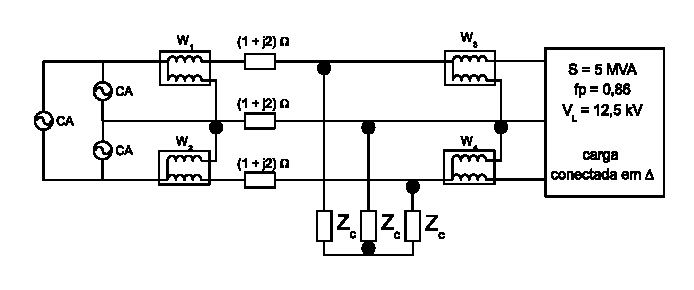
\includegraphics[scale=1]{figuras/circuito.eps}
	
	{Fonte: Elaboração do autor}
\end{figure}


\subsubsection{Objetivos Específicos}

Os principais tópicos são:

\begin{itemize}
\item Utilizar a ferramenta \LaTeX;
\item Inserir equações, tabelas e figuras;
\item Referenciar outros autores de modo correto;
\item Trabalhar com os modelos proposto, bem como o modelo de relatório padrão para trabalhos de conclusão de curso.
\end{itemize}

\section{Fundamentação Teórica}
Nesta seção são mostrados os modos básicos para inserir equações, tabelas e figuras.

\begin{enumerate}
\item item 1
\item item 2
\begin{enumerate}
\item subitem 2.1
\item subitem 2.2
\end{enumerate}
\end{enumerate}

\begin{itemize}
\item Equações

Considere uma rede elétrica $V_a^{2a} = \sqrt{2}$ em regime permanente e as formas de tensão e corrente escritas, respectivamente, nas equações (\ref{Eq:tensao}) e (\ref{Eq:corrente}). Essas equações podem ser encontradas em \cite{nilsson}.


	\begin{equation}
		\left[ {\begin{array}{*{20}{c}}
				a&b&c\\
				f&e&d\\
				g&h&i
		\end{array}} \right]\mu A + \delta i = \lambda {e^2}\sum {x\left[ n \right]} 
		\label{Eq:tensao}
	\end{equation}


\begin{equation}
i(t)=I_{max} \cos(\omega t + \theta_i)=\sqrt{2} I \cos(\omega t + \theta_i) [A]
\label{Eq:corrente}
\end{equation}

\item Tabelas 

Na Tabela \ref{Tab:carga1} e Tabela \ref{Tab:carga2} são mostrados dois conjuntos de cargas de uma empresa industrial, que possuem baixo fator de potência.

\begin{table}[H]
	\centering 
	\caption{Conjunto de cargas da empresa 2}
	\begin{tabular}{ccccc}
		\hline
		& \textbf{Carga 1} & \textbf{Carga 2} & \textbf{Carga 3} & \textbf{Carga 4} \\ \hline
		Potência Ativa (W) & 1200 & 900 & 1000 & 900 \\ \hline
		Fator de Potência & 0,82 & 0,96 & 0,8 & 0,85 \\ \hline
	\end{tabular}
	\label{Tab:carga1}
\end{table}

\begin{table}[H]
\centering 
\caption{Conjunto de cargas da empresa 2}
\begin{tabular}{ccccc}
\hline
& \textbf{Carga 1} & \textbf{Carga 2} & \textbf{Carga 3} & \textbf{Carga 4} \\ \hline
Potência Ativa (W) & 1200 & 900 & 1000 & 900 \\ \hline
Fator de Potência & 0,82 & 0,96 & 0,8 & 0,85 \\ \hline
\end{tabular}
\label{Tab:carga2}
\end{table}

\item Figuras

Na Figura \ref{Fig:circuito} é definido um exemplo de um circuito com fonte e carga conectadas em delta. Também são mostradas os esquemas de ligação para leitura de potência ativa pelo método dos wattímetros.

\begin{figure}[ht!]
\centering
\caption{Modelo de um circuito trifásico \label{Fig:circuito}}
\vspace{-0.5cm}
%fasdfasdf
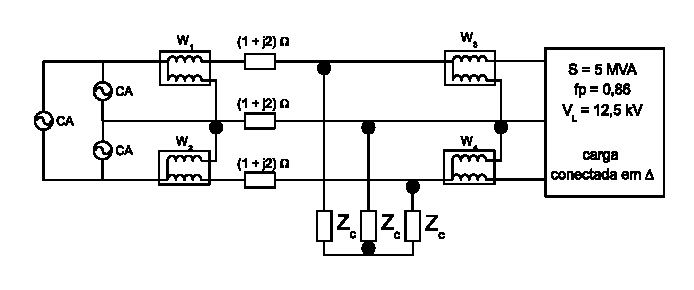
\includegraphics[scale=1]{figuras/circuito.eps}

{Fonte: Elaboração do autor}
\end{figure}
\end{itemize}

\section{Conclusões}
O texto foi produzido pelo professor, afim de mostrar exemplos de como irá ficar o modelo de relatório após a impressão.

Esse modelo é uma proposta para implementação no curso de Engenharia Elétrica da UNOESC, porém pode-se difundir para outros cursos da UNOESC e até mesmo em outras universidades.

\bibliographystyle{abnt-alf}
\bibliography{bibliografia}

\end{document}